\begin{figure}[H]
\centering
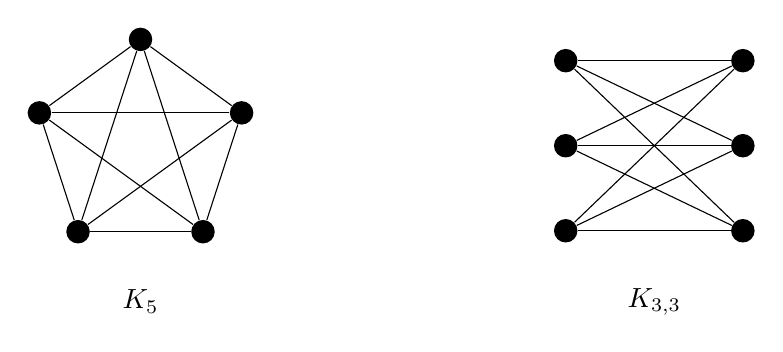
\begin{tikzpicture}[vertex/.style={circle,fill=black,inner sep=3pt}, scale=0.9]
    % K5
    \foreach \i in {0,1,2,3,4} {
        \node[vertex] (k5\i) at ({90+\i*72}:1.5) {};
    }
    \foreach \i in {0,1,2,3,4} {
        \foreach \j in {0,1,2,3,4} {
            \ifnum\i<\j
                \draw (k5\i) -- (k5\j);
            \fi
        }
    }
    \node at (0,-2.2) {$K_5$};
    
    % K_{3,3}
    \begin{scope}[xshift=6cm]
        \node[vertex] (a1) at (0,1.2) {};
        \node[vertex] (a2) at (0,0) {};
        \node[vertex] (a3) at (0,-1.2) {};
        \node[vertex] (b1) at (2.5,1.2) {};
        \node[vertex] (b2) at (2.5,0) {};
        \node[vertex] (b3) at (2.5,-1.2) {};
        \foreach \i in {1,2,3} {
            \foreach \j in {1,2,3} {
                \draw (a\i) -- (b\j);
            }
        }
        \node at (1.25,-2.2) {$K_{3,3}$};
    \end{scope}
\end{tikzpicture}
\caption{The two forbidden minors for planar graphs}
\label{fig:forbidden-planar}
\end{figure}